\documentclass[9pt, aspectratio=169]{beamer}
\usepackage{FiraSans}
\usetheme{metropolis}
\usepackage[utf8]{inputenc}
\usepackage{amsmath}
\usepackage{amsfonts}
\usepackage{amssymb}
\usepackage{multicol}
\usepackage{tikz}
\usetikzlibrary{matrix}
\usepackage{xcolor}
\usepackage[T1]{fontenc} 
\usepackage[skins]{tcolorbox}
\author{Nicola Roman\`o - nicola.romano@ed.ac.uk}
\title{Edge detection and noise reduction methods}
\setlength{\fboxsep}{0pt}
\setbeamertemplate{caption}{\raggedright\insertcaption\par}
\setbeamertemplate {footline}{\begin{scriptsize}\hfill\insertframenumber ~of \inserttotalframenumber\kern1em\vskip5pt\end{scriptsize}}

%\setbeamercovered{transparent} 
%\setbeamertemplate{navigation symbols}{} 

\titlegraphic{\centering 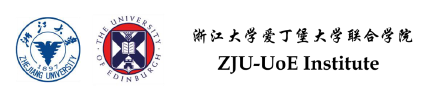
\includegraphics[scale=.5]{instituteLogo.png}}
\date{}

\AtBeginSection[]
{
  \begin{frame}<beamer>
    {Outline}
    \huge{\tableofcontents[currentsection]}
  \end{frame}
}

\begin{document}

\newtcolorbox{codebox}{enhanced,
    top=2pt,
    left=2pt,
    right=2pt,
    bottom=2pt,
    boxrule=0pt,
    leftrule=5pt,
    sharp corners,
    colback=gray!20,
    colframe=blue!60!black}

\begin{frame}
    \titlepage
\end{frame}

\begin{frame}
    {Learning objectives}
    \begin{columns}
        \begin{column}{0.8\textwidth}
            \begin{itemize}
                \item Explain the use of image gradients for edge detection.
                \item Describe various edge detection algorithms and how they work.
                \item Describe different noise reduction algorithms and how they work.
                \item Use Scikit Image to implement these techniques.
            \end{itemize}
        \end{column}
        \begin{column}{0.2\textwidth}
            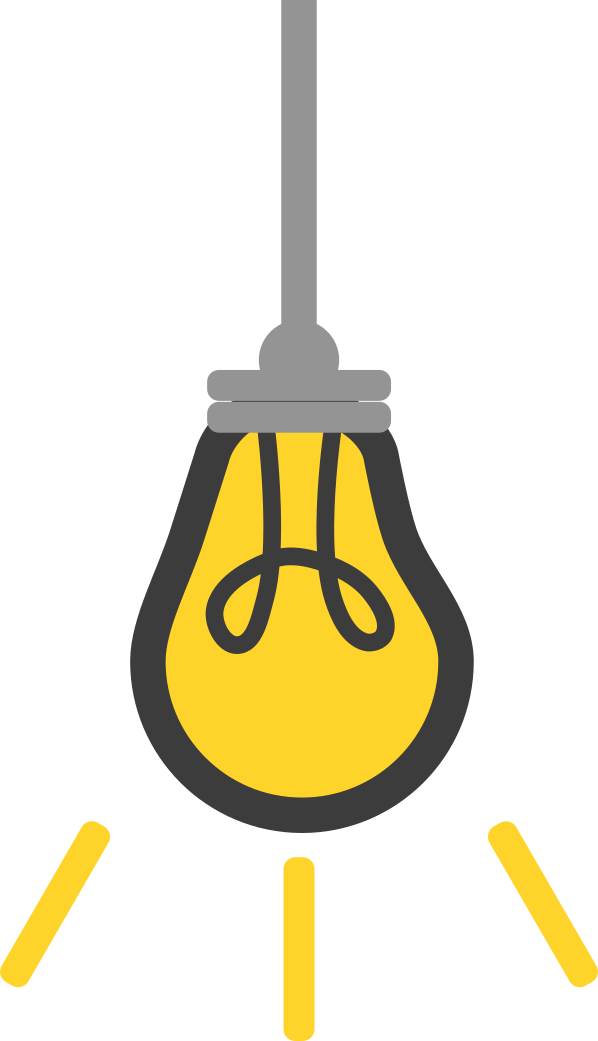
\includegraphics[angle=-30, origin=tr, width=1.5\textwidth]{lightbulb.png}
        \end{column}
    \end{columns}
\end{frame}

\section{Edge detection - introduction}

\begin{frame}
    {Edge detection problem}
    An edge is an area where the brightness of an image changes more or less gradually.

    Detecting edges is useful e.g. to find objects in a scene, determine which pixels belong to which objects, and measure their properties.
    \begin{figure}
        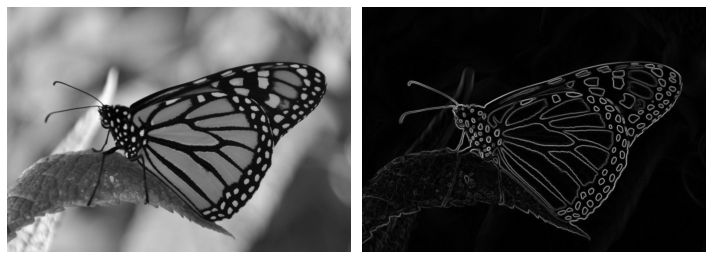
\includegraphics[width=\textwidth]{monarch_sobel.png}
        \caption{\footnotesize{\color{gray}{Monarch butterfly - CC-BY-SA 2.0 Ted @ Flickr}\color{black}}}
    \end{figure}
\end{frame}

\begin{frame}
    {How to detect an edge?}
    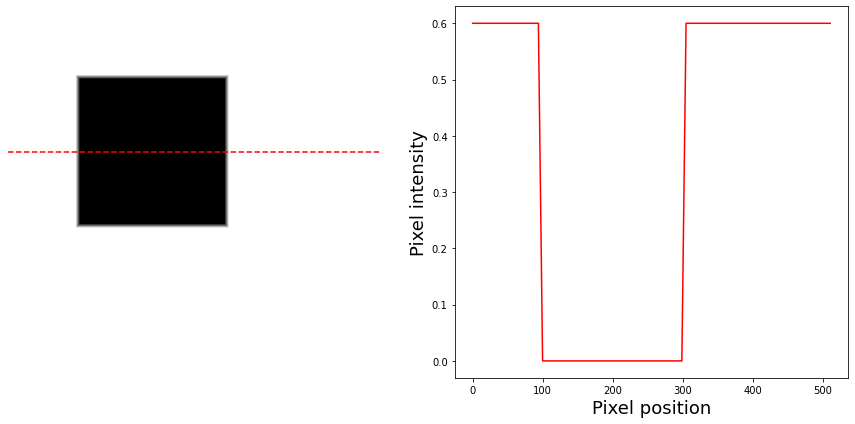
\includegraphics[width=\textwidth]{line_intensity.png}
    Consider the vertical edges. We can see a change in the intensity of pixels as we move from black to white and vice versa. \textbf{Can you think of a way to detect these edges?}
\end{frame}

\subsection{Derivatives}

\begin{frame}
    {We can use derivatives!}
    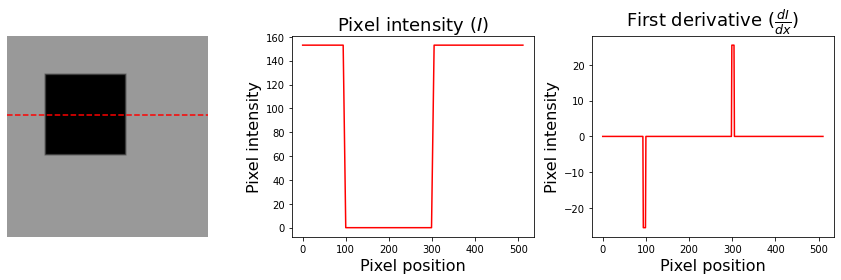
\includegraphics[width=\textwidth]{intensity_derivative.png}
    Edges will correspond to minima and maxima of the derivative of the intensity!
\end{frame}

\begin{frame}
    {Image derivatives}
    With a 2D image, we can find the x and y derivatives of the image intensity.

    The vector of derivatives is called the \textbf{gradient} and is given by:
    \Large
    $$\nabla I = \begin{bmatrix}\frac{\partial I}{\partial x}, \frac{\partial I}{\partial y}\end{bmatrix}$$

    \normalsize

    The gradient is a vector with:
    \begin{itemize}
        \item Direction perpendicular to the edge
              $$\theta = \arctan\left(\frac{\partial I}{\partial x} \mathbin{/} \frac{\partial I}{\partial y}\right)$$
              \pause
        \item Length (\textbf{gradient magnitude}) proportional to the intensity change
              $$\lvert\lvert\nabla I\rvert\rvert = \sqrt{\left(\frac{\partial I}{\partial x}\right)^2 + \left(\frac{\partial I}{\partial y}\right)^2}$$
    \end{itemize}
\end{frame}

\begin{frame}
    {Example of gradient vectors}
    \centering
    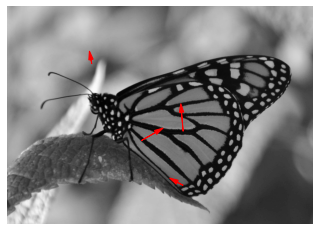
\includegraphics[width=.7\textwidth]{monarch_gradient.png}
\end{frame}

\subsection {Calculating derivatives}

\begin{frame}
    {Calculating a discrete derivative}
    How to calculate a discrete derivative?

    Remember the definition of a derivative for a continuous function $f(x)$:
    $$f'(x) = \frac{df}{dx} = \lim_{\Delta x \rightarrow 0} \frac{f(x) - f(x - \Delta x)}{\Delta x}$$

    \pause
    Our image is not continuous, as it is made up of discrete pixels so the minimum $\Delta x$ value is 1 (a single pixel).

    \pause
    The discrete derivative is given by:
    $$\frac{dI}{dx} = \frac{I(x) - I(x-1)}{1} = I(x) - I(x-1)$$
\end{frame}

\begin{frame}
    {Calculating the discrete derivative - variations}
    We can choose to calculate the discrete derivative in three different ways

    \Large
    \begin{itemize}
        \item \textbf{Forward difference}: $I(x) - I(x+1)$
        \item \textbf{Backward difference}: $I(x) - I(x-1)$
        \item \textbf{Central difference}: $I(x+1) - I(x-1)$
    \end{itemize}

    \pause
    These can be easily calculated using \textbf{convolution}!

    \begin{itemize}
        \item \textbf{Forward difference}: $\begin{bmatrix}1&-1\end{bmatrix}$
        \item \textbf{Backward difference}: $\begin{bmatrix}-1&1\end{bmatrix}$
        \item \textbf{Central difference}: $\begin{bmatrix}-1&0&1\end{bmatrix}$
    \end{itemize}
\end{frame}

\begin{frame}
    {Discrete derivative - example}
    Let's calculate the discrete derivative of this 1D image using central difference

    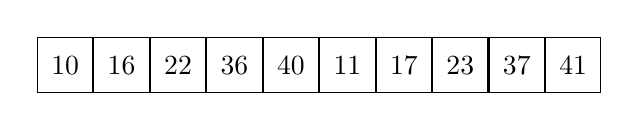
\begin{tikzpicture}[ampersand replacement=\&]
        \matrix [matrix of nodes, nodes={draw, minimum height=2em, minimum width=2em, anchor=center}, column sep=0] at (0, 0) {10 \& 16 \& 22 \& 36 \& 40 \& 11 \& 17 \& 23 \& 37 \& 41\\};
    \end{tikzpicture}

    \pause
    Convolving with the kernel

    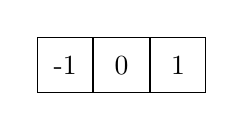
\begin{tikzpicture}[ampersand replacement=\&]
        \matrix [matrix of nodes, nodes={draw, minimum height=2em, minimum width=2em, anchor=center}, column sep=0] at (0, 0) {-1 \& 0 \& 1\\};
    \end{tikzpicture}

    We obtain the following

    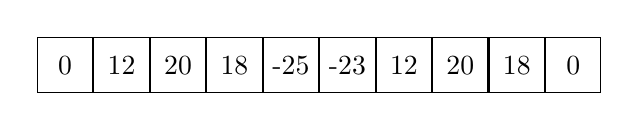
\begin{tikzpicture}[ampersand replacement=\&]
        \matrix [matrix of nodes, nodes={draw, minimum height=2em, minimum width=2em, anchor=center}, column sep=0] at (0, 0) {0 \& 12 \& 20 \& 18 \& -25 \& -23 \& 12 \& 20 \& 18 \& 0\\};
    \end{tikzpicture}
\end{frame}

\begin{frame}
    {Derivative of an image}
    We can apply these convolution kernels to an image as well.

    $$K_x = \begin{bmatrix}-1&0&1\end{bmatrix} \qquad K_y = \begin{bmatrix}-1\\0\\1\end{bmatrix}$$

    \centering
    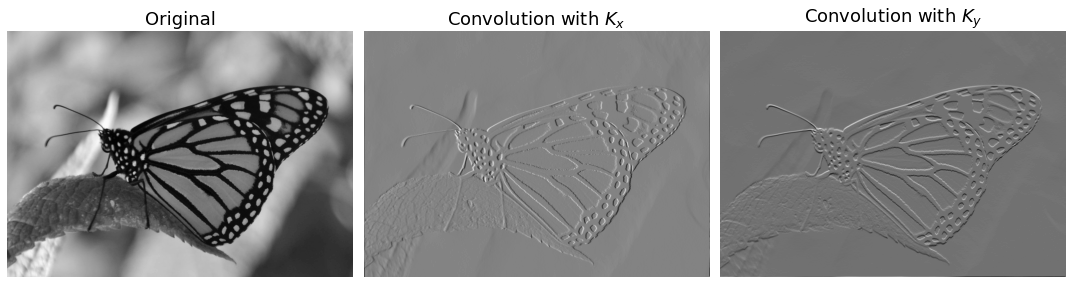
\includegraphics[width=.8\textwidth]{monarch_derivatives.png}
\end{frame}

\begin{frame}
    {The problem with noise...}
    Derivatives are very sensitive to noise. Smoothing the function beforehand helps

    \centering
    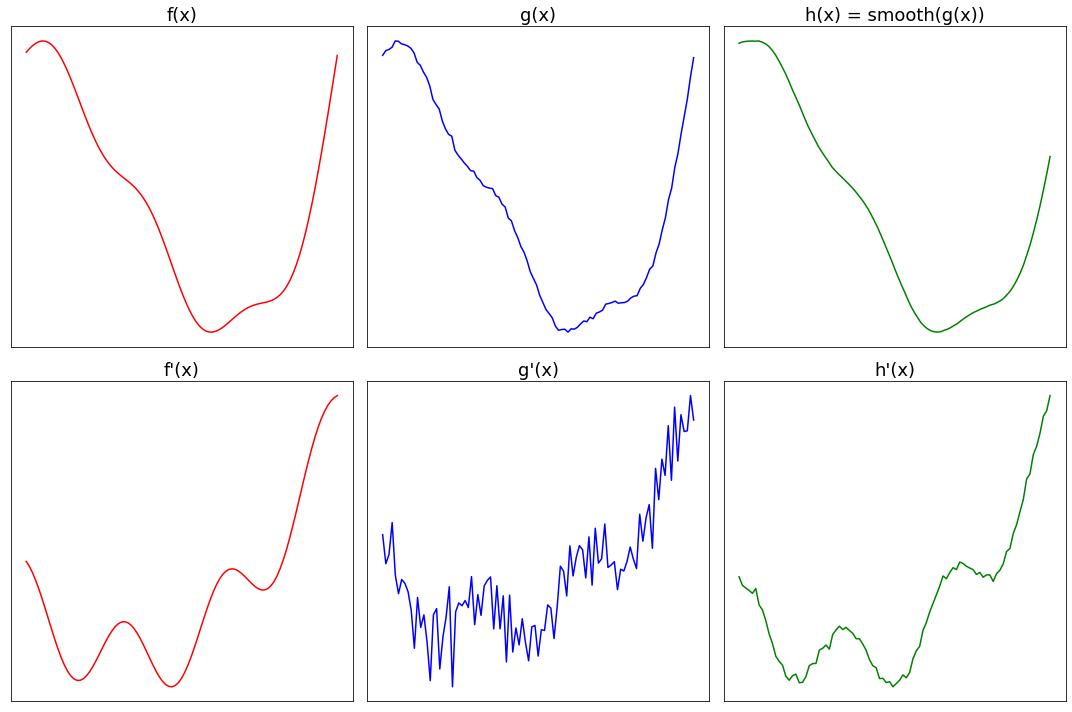
\includegraphics[width=.7\textwidth]{derivative_noise.png}
\end{frame}

\section{Edge detection algorithms}
\subsection{Prewitt and Sobel}

\begin{frame}
    {2D derivative kernels (Prewitt edge detectors)}
    Expanding the derivative kernels to 2D we can directly smooth our intensity function.

    These are called \textbf{Prewitt} kernels.

    $$K_x = \begin{bmatrix}-1&0&1\\-1&0&1\\-1&0&1\end{bmatrix} \qquad K_y = \begin{bmatrix}-1&-1&-1\\0&0&0\\1&1&1\end{bmatrix}$$

    Alternatively the \textbf{Sobel} kernels can be used:

    $$K_x = \begin{bmatrix}-1&0&1\\-2&0&2\\-1&0&1\end{bmatrix} \qquad K_y = \begin{bmatrix}-1&-2&-1\\0&0&0\\1&2&1\end{bmatrix}$$
\end{frame}

\begin{frame}
    {Your turn!}
    Consider the following image. \textbf{What do you expect to obtain and why} after convolution with the Prewitt kernels?\\
    Apply the convolution (you can easily do that by hand); \textbf{do the results match} your prediction?

    $$\begin{bmatrix}0   & 0   & 0   & 0   & 0   & 0   & 0   & 0   \\
            0   & 0   & 0   & 0   & 0   & 0   & 0   & 0   \\
            0   & 0   & 0   & 0   & 0   & 0   & 0   & 0   \\
            50  & 50  & 50  & 50  & 50  & 50  & 50  & 50  \\
            100 & 100 & 100 & 100 & 100 & 100 & 100 & 100 \\
            100 & 100 & 100 & 100 & 100 & 100 & 100 & 100 \\
            50  & 50  & 50  & 50  & 50  & 50  & 50  & 50  \\
            0   & 0   & 0   & 0   & 0   & 0   & 0   & 0   \\
            0   & 0   & 0   & 0   & 0   & 0   & 0   & 0
        \end{bmatrix}$$
\end{frame}

\begin{frame}
    {Edge detection - Prewitt and Sobel}
    Having applied either the Prewitt or Sobel kernels to the image we can now detect edges.

    Simply threshold the gradient magnitude of the image to define which pixels are edges.

    \centering
    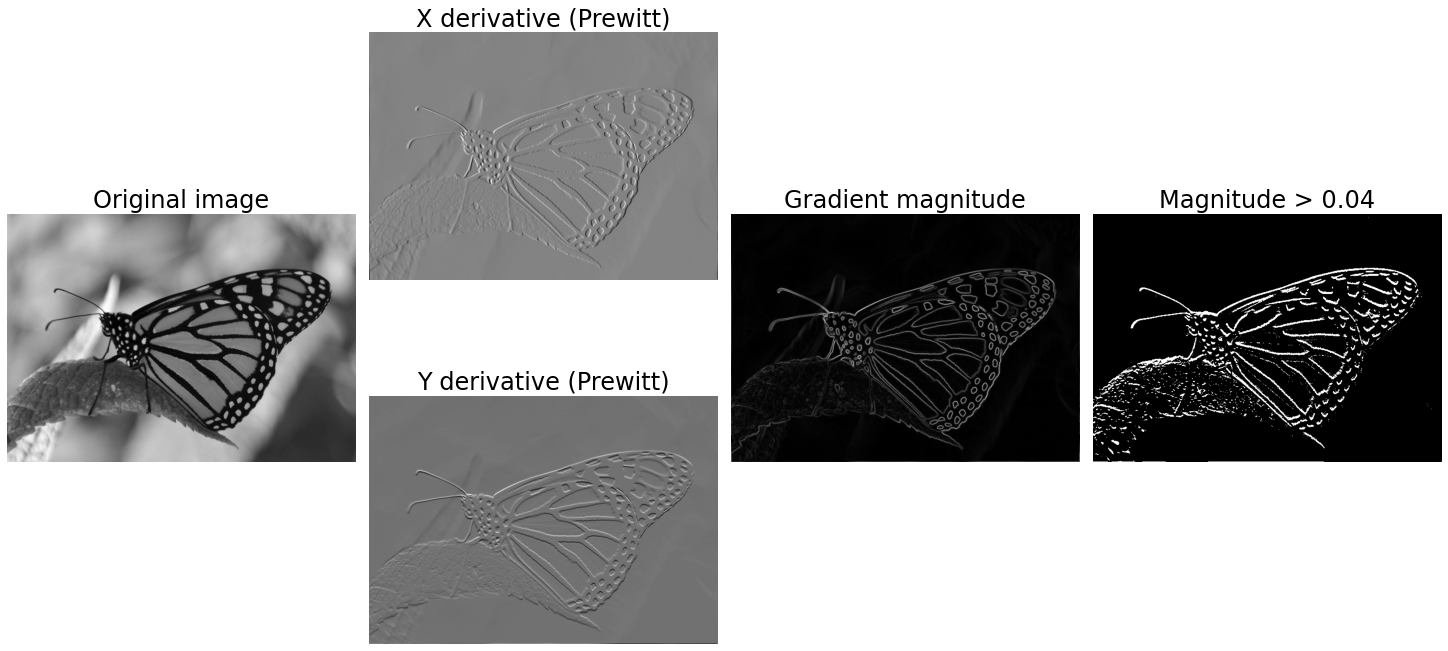
\includegraphics[width=.9\textwidth]{monarch_prewitt.png}
\end{frame}

\begin{frame}
    {Edge detection in Scikit Image}
    \begin{columns}
        \begin{column}{.6\textwidth}
            \begin{codebox}
                \texttt{from skimage.filters import prewitt, sobel\\
                    from skimage.io import imread\\
                    \\
                    img = imread("butterfly.jpg")\\
                    im\_prewitt = prewitt(img)\\
                    im\_sobel = sobel(img)\\
                    \pause
                    \\
                    fig, ax = plt.subplots(2, 1, figsize=(5, 10))\\
                    ax[0].imshow(im\_prewitt > 0.08, cmap="gray")\\
                    ax[0].set\_title("Prewitt", fontsize=25)\\
                    ax[1].imshow(im\_sobel > 0.08, cmap="gray")\\
                    ax[1].set\_title("Sobel", fontsize=25)\\
                    for a in ax:\\
                    a.axis("off")\\
                    plt.show()}
            \end{codebox}
        \end{column}
        \begin{column}{.4\textwidth}
            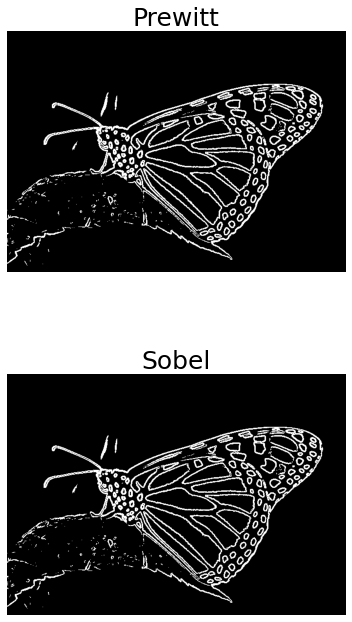
\includegraphics[width=.7\textwidth]{monarch_prewitt_sobel.png}
        \end{column}
    \end{columns}
\end{frame}

% \subsection{Marr-Hildreth}

% \begin{frame}
%     {Marr-Hildreth detector (Laplacian of Gaussian)}

%     The Marr-Hildreth detector finds edges by first smoothing the image using a Gaussian filter, then finding the Laplacian of the smoothed image.

%     \pause

%     The Laplacian ($\Delta$ or $\nabla^2$) of the image is the sum of the second partial derivatives of the image.

%     $$\nabla^2(I) = \frac{\partial^2 I}{\partial x^2} + \frac{\partial^2 I}{\partial y^2}$$

%     Technically, this is defined as the divergence of the gradient of the image. 

% \end{frame}

\subsection {Canny}
\begin{frame}
    {The Canny edge detector}
    The Canny edge detector is a more advanced algorithm to detect edges.

    It involves five steps

    \begin{enumerate}
        \item Apply a Gaussian filter to the image to smooth out noise
        \item Calculate the gradient magnitude (e.g. using a Sobel filter)
        \item Non-maximum suppression
        \item Double thresholding
        \item Edge tracking by hysteresis
    \end{enumerate}
\end{frame}

\begin{frame}
    {The Canny edge detector - step 1 and 2 - smoothing and gradient}
    We start by convolving the image with a Gaussian kernel to smooth noise.

    We then calculate the gradient magnitude and angle using the Sobel kernels.
    \centering
    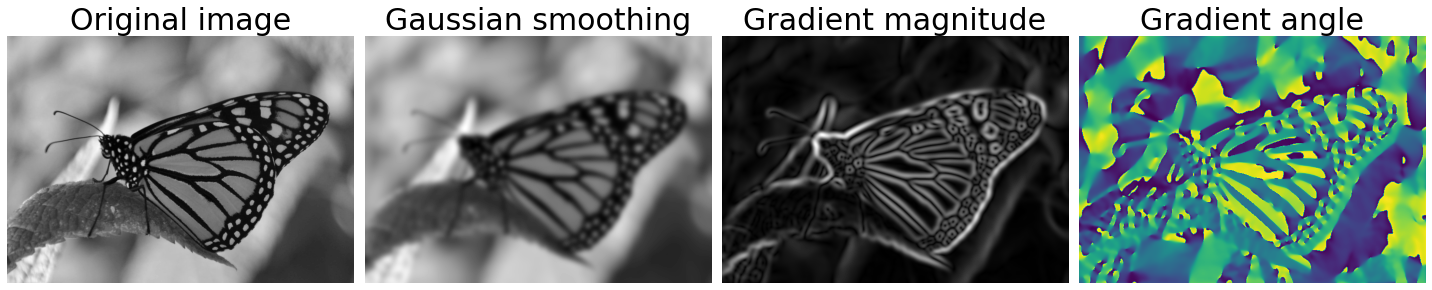
\includegraphics[width=\textwidth]{canny_step1-2.png}
\end{frame}

\begin{frame}
    {The Canny edge detector - step 3 - non-maximum suppression}
    Non-maximum suppression allows us to thin the edges by only keeping the pixels with the largest gradient magnitude in the edge.

    For each pixel, we take the neighbouring pixels in the direction of the gradients, and we keep only the pixels with the largest gradient magnitude.

    \begin{columns}
        \begin{column}{.33\textwidth}
            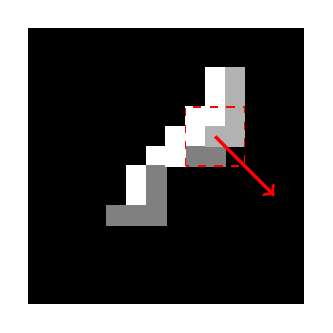
\begin{tikzpicture}[scale=0.25]
                \draw [fill=black] (-5, -5) rectangle (9, 9);
                \draw [fill=white, color=white] (0, 0) rectangle (1, 2) rectangle (2, 3) rectangle (4, 4) rectangle (5, 6) rectangle (4, 7);
                \draw [fill=white, color=white] (3, 4) rectangle (4, 5);
                \draw [fill=gray, color=gray] (-1, -1) rectangle (2, 0) rectangle (1, 2);
                \draw [fill=gray, color=gray] (2, 2) rectangle (5, 3);
                \draw [fill=black!30!white, color=black!30!white] (4, 3) rectangle (6, 4) rectangle (5, 7);
                \draw [fill=white, color=white] (2, 2) rectangle (3, 3);
                \draw [->, color=red, very thick] (4.5, 3.5) -- (7.5, 0.5);
                \draw [color=red, dashed] (3, 2) rectangle (6, 5);
            \end{tikzpicture}
        \end{column}
        \begin{column}{.33\textwidth}
            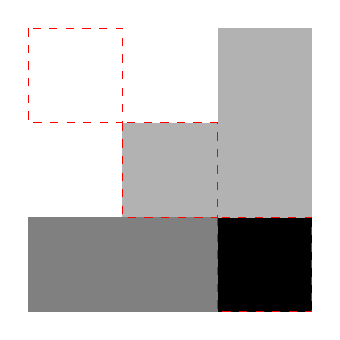
\begin{tikzpicture}[scale=1.2]
                \draw [fill=black] (0, 0) rectangle (3, 3);
                \draw [fill=white, color=white] (0, 1) rectangle (1, 2);
                \draw [fill=black!30!white, color=black!30!white] (1, 1) rectangle (3, 3);
                \draw [fill=white, color=white] (0, 2) rectangle (2, 3);
                \draw [fill=gray, color=gray] (0, 0) rectangle (2, 1);
                \draw [color=red, dashed] (0, 3) rectangle (1, 2) rectangle (2, 1) rectangle (3, 0);
            \end{tikzpicture}
        \end{column}
        \pause
        \begin{column}{.33\textwidth}
            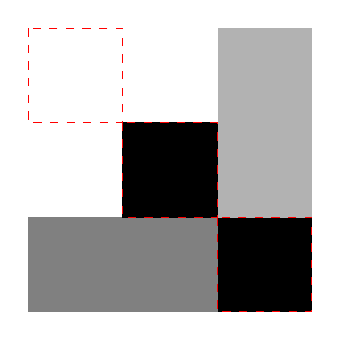
\begin{tikzpicture}[scale=1.2]
                \draw [fill=black] (0, 0) rectangle (3, 3);
                \draw [fill=white, color=white] (0, 1) rectangle (1, 2);
                \draw [fill=black!30!white, color=black!30!white] (1, 1) rectangle (3, 3);
                \draw [fill=white, color=white] (0, 2) rectangle (2, 3);
                \draw [fill=gray, color=gray] (0, 0) rectangle (2, 1);
                \draw [fill=black, color=black] (1, 1) rectangle (2, 2);
                \draw [color=red, dashed] (0, 3) rectangle (1, 2) rectangle (2, 1) rectangle (3, 0);
            \end{tikzpicture}
        \end{column}
    \end{columns}
\end{frame}

\begin{frame}
    {The Canny edge detector - step 4 - double thresholding}
    The next step is to set two arbitrary thresholds, one for the weak edges and one for the strong edges.

    \begin{itemize}
        \item \textbf{Strong edges} are those with gradient magnitude above the high threshold.
        \item \textbf{Weak edges} are those with gradient magnitude between the low and high threshold.
        \item Edges with gradient magnitude below the low threshold are suppressed (set to 0).
    \end{itemize}
\end{frame}

\begin{frame}
{The Canny edge detector - step 5 - hysteresis}
We need to decide what to do with weak edges.
We keep those weak edges that are near a strong edge, and discard the others.

\vspace{2em}

\begin{columns}
    \begin{column}{.33\textwidth}
        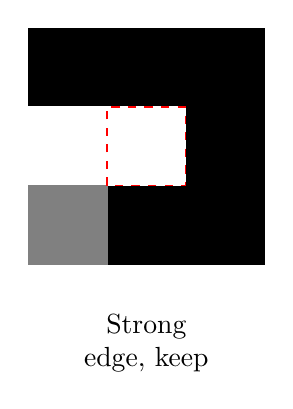
\begin{tikzpicture}
            \draw [fill=black] (0, 0) rectangle (3, 3);
            \draw [fill=white, color=white] (0, 1) rectangle (2, 2);
            \draw [fill=gray, color=gray] (0, 0) rectangle (1, 1);
            \draw [color=red, dashed] (1, 1) rectangle (2, 2);
            \node [align=center, text width=2cm] at (1.5, -1) {Strong edge, keep};
        \end{tikzpicture}
    \end{column}
    \begin{column}{.33\textwidth}
        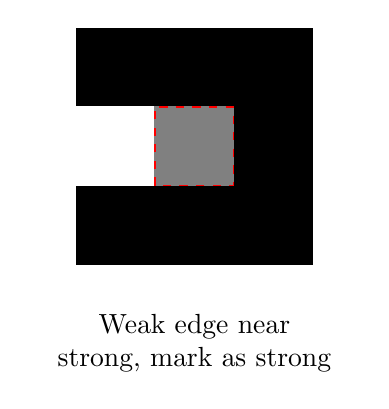
\begin{tikzpicture}
            \draw [fill=black] (0, 0) rectangle (3, 3);
            \draw [fill=white, color=white] (0, 1) rectangle (1, 2);
            \draw [fill=gray, color=gray] (1, 1) rectangle (2, 2);
            \draw [color=red, dashed] (1, 1) rectangle (2, 2);
            \node [align=center, text width=4cm] at (1.5, -1) {Weak edge near strong, mark as strong};
        \end{tikzpicture}
    \end{column}
    \begin{column}{.33\textwidth}
        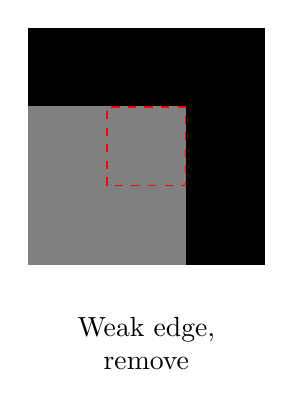
\begin{tikzpicture}
            \draw [fill=black] (0, 0) rectangle (3, 3);                
            \draw [fill=gray, color=gray] (0, 0) rectangle (2, 2);
            \draw [color=red, dashed] (1, 1) rectangle (2, 2);
            \node [align=center, text width=2cm] at (1.5, -1) {Weak edge, remove};
        \end{tikzpicture}
    \end{column}
\end{columns}
\end{frame}

\begin{frame}
{The Canny edge detector - The final result!}
\centering
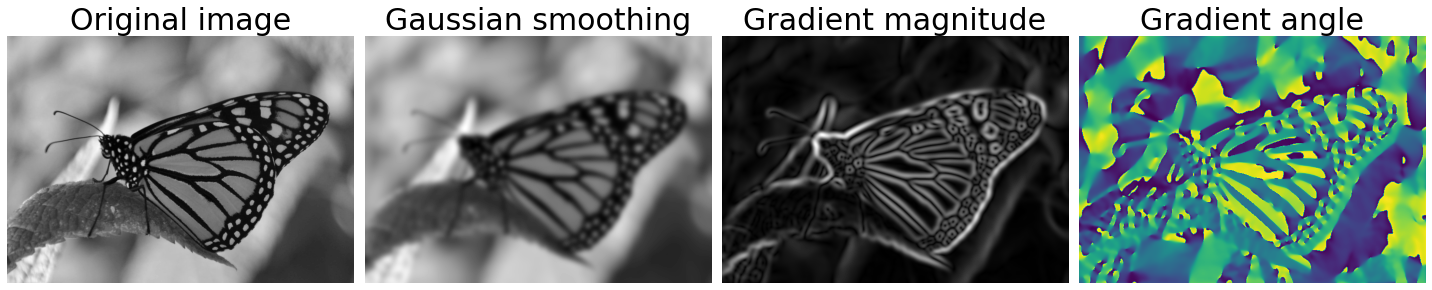
\includegraphics[width=\textwidth]{canny_step1-2.png}

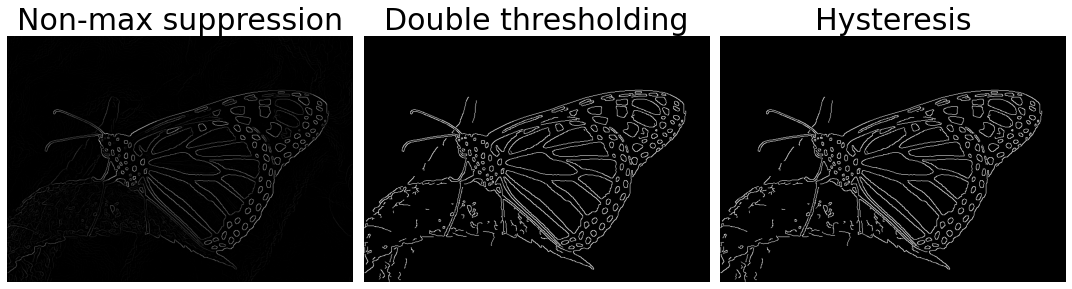
\includegraphics[width=.75\textwidth]{canny_step3-5.png}

All these steps are implemented in the \href{https://scikit-image.org/docs/dev/api/skimage.feature.html\#skimage.feature.canny}{\underline{skimage.feature.canny}} function.
Try it by yourself and change the parameters to see what happens!
\end{frame}
\end{document}